\section{Model Exercise 1-1 (05): Swelling of red salt clay}
\label{sec:mex05}
%------------------------------------------------------------------------------
\Authors{Amir Sattari, Keita Yoshioka, Mathias Nest, Christopher R\"olke}
%------------------------------------------------------------------------------
Model Exercise (MEX 1-1) investigates the closure of micro pathways by swelling of red salt clay. The numerical and experimental approaches are considered to understand the governing factors, which result in materials behavior change during the swelling process. The experimental setup is described in section \ref{sec:t4swell}.

\subsection{Experiment}

\begin{figure}[ht]
\centering
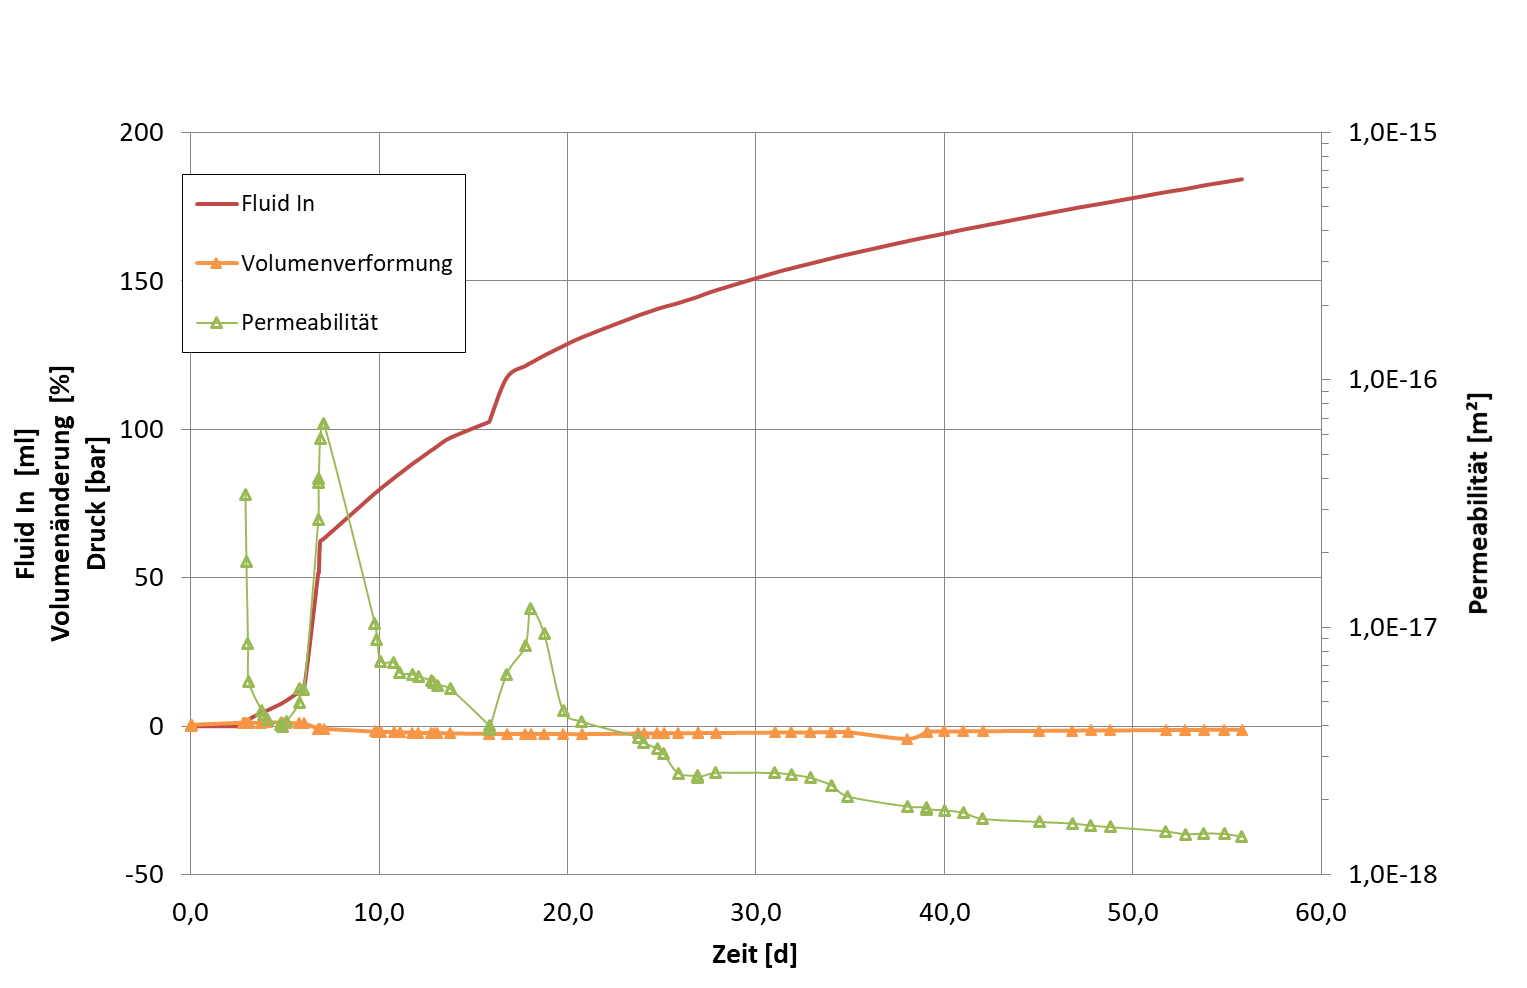
\includegraphics[width=0.8\textwidth]{figures/IfG-T4-results.png}
\caption{Results of the 8 week swelling test of T4 clay.}
\label{fig:t4swellresults}
\end{figure}

The experiment was conducted on a sample of dry red salt clay from the Aller series (T4) of the Zechstein in northern Germany. The experiment ran for 8 weeks, under isostatic stress conditions of 4 bar, and a brine pressure of 1 bar. 

Figure \ref{fig:t4swellresults} shows the amount of fluid that went into the sample (red), the change of the volume of the medium which applies the surrounding pressure (orange), and the permeability (green). We see that during the first three weeks the brine modifies the clay, and pathways are opened and closed. Apart from the wetting of the clay this may also be due to some salt going into solution and recrystallization. After this the permeability behaves more smoothly, and decreases with time. At all times the volume of the surrounding medium was below its initial value, indicating that swelling took place. 

%------------------------------------------------------------------------------


%------------------------------------------------------------------------------
\subsection{Model approach}
\subsubsection*{Lattice element model}

With the application of the lattice model, the simulation of the swelling process in red salt clay sample is investigated. The experimental data provided by IfG Leipzig are used to determine the initial permeability and hydraulic aperture values. The calculated parameters then are transformed into lattice model to simulate the swelling and change of the permeability with swelling process. The salt re-crystallization and closure of micro-pathways is not investigated here. The expansion of the elements based on the shrinkage and swelling model described in section \ref{Section:ShrinkageLattice} is carried out. The expansion of the elements results in decrease of the hydraulic aperture and therefore lower permeability values. However, during the swelling process the micro fracking is also observed. The elements expansion lead to higher axial confinement stresses between the Voronoi cells, which is represented by interface elements.  Eventually, the outcome of the simulation is compared to the experimental results. 

\todo[inline]{[CAU] Please add LEM results}
\todo[inline]{[UFZ] Keita will you contribute to this MEX?}

%------------------------------------------------------------------------------
\subsection{Results and discussion}